%\documentstyle[a4j,epsbox,graphicx]{jarticle}
\documentclass[a4j]{jarticle}%変更禁止!
%%%%%%%%%%%%usepackageは適宜追加してください.%%%%%%%%%%%%%%%%%%%%%%%%%%%%%%%%%%%%%%%%%%%%%%%%%%%
%\usepackage{epsbox}
%\usepackage{graphicx}
\usepackage[dvipdfmx]{graphicx,color}

\newcommand\figref[1]{\textbf{図~\ref{fig:#1}}}
\newcommand\tabref[1]{\textbf{表~\ref{tab:#1}}}
% \renewcommand{\labelnamepunct}{\addcolon\addspace}
% \renewbibmacro{in:}{}
%%%%%%%%%%%%%%%%%%%%%%%%%%%ここから変更禁止%%%%%%%%%%%%%%%%%%%%%%%%%%%%%%%%%%%%%%%%%%%%%%%%%%
\topmargin -28mm
\oddsidemargin -15mm
\evensidemargin -15mm
\textwidth 185mm
\textheight 275mm
\columnsep 6mm

%\def\toujitu{Dec. 2020}

\makeatletter
\def\section{\@startsection{section}{2}{\z@}{.8ex plus .8ex minus 
 .2ex}{.05ex plus .07ex}{\large\bf}}
\makeatother
\makeatletter
\def\subsection{\@startsection{subsection}{2}{\z@}{.8ex plus .8ex minus 
 .2ex}{.05ex plus .07ex}{\bf}}
\makeatother


\pagestyle{empty}

\begin{document}

\baselineskip 4.75mm

\twocolumn
[
  \footnotesize
  \begin{center}
    {~}\\
    %\begin{center}
    %{ユビキタスウェアラブルワークショップ2020 
    %\hfill \toujitu}\\
    %%%%%%%%%%%%%%%%%%%%%%%%%%%ここまで変更禁止%%%%%%%%%%%%%%%%%%%%%%%%%%%%%%%%%%%%%%%%%%%%%%%%%%

    %%%注意!!\vspaceは図表部分のみ見にくく(醜く)ならない範囲内で使用可能とします.%%%%%%%%%%%%%%%%%%%%%%%%%%%%

    \medskip
    {\large
      %タイトル
      {\bf ディスプレイを用いた擬似的脈波生成手法の検討}\\
    }
    \medskip
    {\large
      %著者 同じ所属の人が連続する場合は連続する同じ所属の著者の最後の著者のみに所属を付けること.
      藤井敦寛(立命館大学),村尾和哉(立命館大学,JSTさきがけ)
    }
  \end{center}
]

\section{研究の背景と目的}
% 近年,健康管理への意識の高まりから,自身の生体情報を記録するウェアラブルデバイスが広く普及している.記録する生体情報は活動量や呼吸数,体温など様々な情報があり,心拍数もその一つである.心拍数を取得するために用いられる脈波センサでは,緑色のLEDを皮膚に照射して,反射した光の変化から脈波を計測する光電式容積脈波記録法(PPG)と呼ばれる方式のものが一般的であり,スマートウォッチにも導入されている.Spinsanteら\cite{accuracy_in_low_intensity}は低強度の身体活動時にスマートウォッチから取得される心拍数に注目し,その精度を計測している.また,スマートウォッチから取得できる心拍データを用いて,今井ら\cite{fatigue_detection}が疲労度を検出する手法を提案している.このほか,Hanら\cite{arrhythmia_detection}は不整脈を検出する手法を提案しており,スマートウォッチから得られる脈波データを使用した研究は盛んである.しかしながら,皮膚内の血管に向けて光を照射するという特性上,センサの装着位置に血管が存在しない場合は使用が不可能である.例えば,義手にスマートウォッチを装着する場合,正常な心拍数が取得できない.市販のスマートウォッチは心拍数データも含めた生体情報を取得し,その変化などからアノテーションを行い,活動記録として残していくものが大半である.そのため,正常な心拍数が取得できない場合は正しい活動が記録されない可能性が高い.
近年,健康管理への意識の高まりから,自身の生体情報を記録するウェアラブルデバイスが広く普及している.記録する生体情報は活動量や呼吸数,体温など様々な情報があり,心拍数もその一つである.心拍数を取得するために用いられる脈波センサでは,緑色のLEDを皮膚に照射して,血管を通して反射した光の変化から脈波を計測する光電式容積脈波記録法(PPG)と呼ばれる方式のものが一般的であり,スマートウォッチにも導入されている.今井ら\cite{fatigue_detection}がスマートウォッチから取得できる心拍データを用いて疲労度を検出する手法を提案しているなど,スマートウォッチから得られる脈波データを使用した研究は盛んである.しかしながら,皮膚内の血管に向けて光を照射するという特性上,センサの装着位置に血管が存在しない場合は使用が不可能である.例えば,義手にスマートウォッチを装着する場合,正常な心拍数が取得できない.多くのスマートウォッチは心拍数データも含めた生体情報を取得し,活動記録
を残す.そのため,正常な心拍数が取得できない場合には,正しい活動が記録されない可能性がある.
\par

任意の脈波を生成することが可能であれば,スマートウォッチを義手などに装着する場合でも,他の身体部位から取得された正しい脈波データを複製し,スマートウォッチに入力することが可能となる.本研究では,ディスプレイを用いて擬似的に脈波データを生成する手法を検討する.あらかじめ収集された実際の脈波データを参考にして,ディスプレイの色調を変化させることで,脈波センサの取得値を意図的に操作する.ディスプレイを用いて擬似的に脈波データを生成することが可能か確認し,提案手法の有効性を明らかにする.


\section{予備実験}
予備実験として,ディスプレイ上に脈波センサを貼り付けた状態で,ディスプレイの色調を変化させたときの脈波センサの取得値を観察した.

\subsection{実験環境}
参考にする脈波データを事前に収集した.被験者は20代男性1名である.\figref{sensors}の左図に示すように,左手人差し指に光電式容積脈波記録法の脈波センサ(pulsesensor.com製)を装着した.脈波センサはArduinoUNOを介してPCに接続しており,サンプリング周波数は約90Hzで10秒間データの収集を行った.
\par

擬似脈波の生成には,データの収集で使用するPCとは異なるPCのディスプレイを使用した.\figref{sensors}の右図に示すように,ディスプレイ上に脈波センサを乗せ,光が入らないように布で覆った後,ガムテープで固定した.事前に脈波データを取得した時と同じ条件でデータの取得を行った.ディスプレイの色調の変化にはJavaScriptを使用し,ブラウザの背景色を変化させることで制御した.事前に収集した脈波データを1サンプルずつ読み込み,その値に応じた3色で表示を繰り返す.全サンプルの処理が終了した場合,同じデータで再び処理を行う.値が685より大きければR:150, G:19, B:20,465より小さければR:157, G:26, B:27,それ以外の場合はR:156, G:25, B:26の色を表示する.また,色の表示ごとに10[ms]の遅延を挟んだ.

\subsection{結果と考察}
取得された脈波データを,最初のピークから5秒間切り出した結果を\figref{pulse}に示す.結果から,波形の形やピークの位置に違いがあることが確認できる.これは,ディスプレイ制御の開始時刻とセンサ値取得の開始時刻を同期していなかったことや,色の表示ごとの遅延を10[ms]に固定していたことが影響したと考えられる.しかしながら,擬似的にピークを生成できていることから,ディスプレイを使用するアプローチは有効だといえる.


\section{まとめと今後}
本研究では,ディスプレイを用いて擬似的に脈波データを生成する手法を実現するために,ディスプレイの色調を変化させることで,脈波センサの取得値を意図的に操作することが可能であるか調査した.今後は,別の身体部位から取得された脈波データをリアルタイムに再現するプログラムを実装する.そのためには,手動ではなく自動でディスプレイの色調を決定し,変化に適応していく必要がある.具体的な実現方法として,ディープラーニングの手法の一つであるLSTM(Long short-term memory)を使用し,直近数秒間のデータを繰り返し入力しながら再現していくことを検討している.


\begin{figure}[!t]
  \begin{center}
    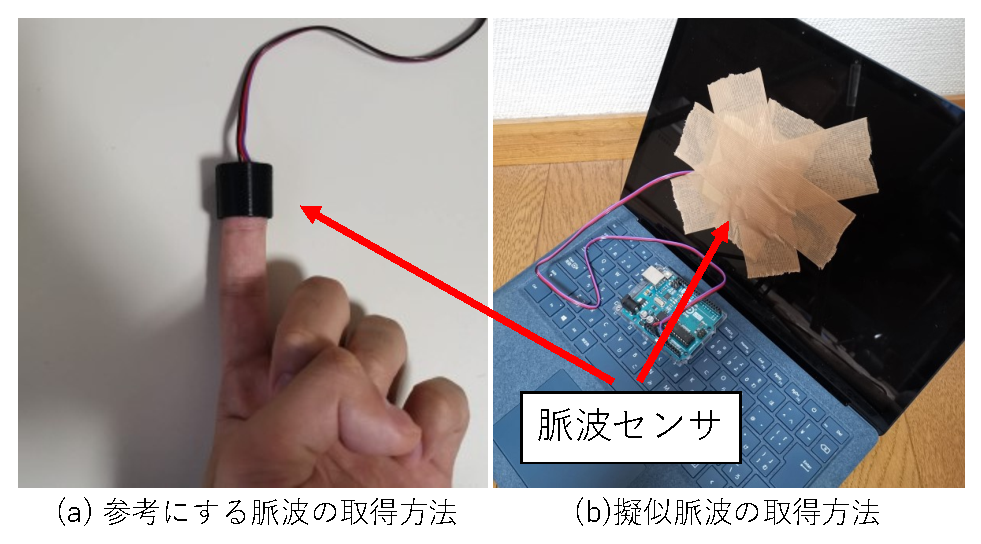
\includegraphics[width=1\linewidth]{sensors.eps}
  \end{center}
  \vspace{-8mm}
  \caption{脈波データの取得方法}
  \label{fig:sensors}
\end{figure}

\begin{figure}[!t]
  \begin{center}
    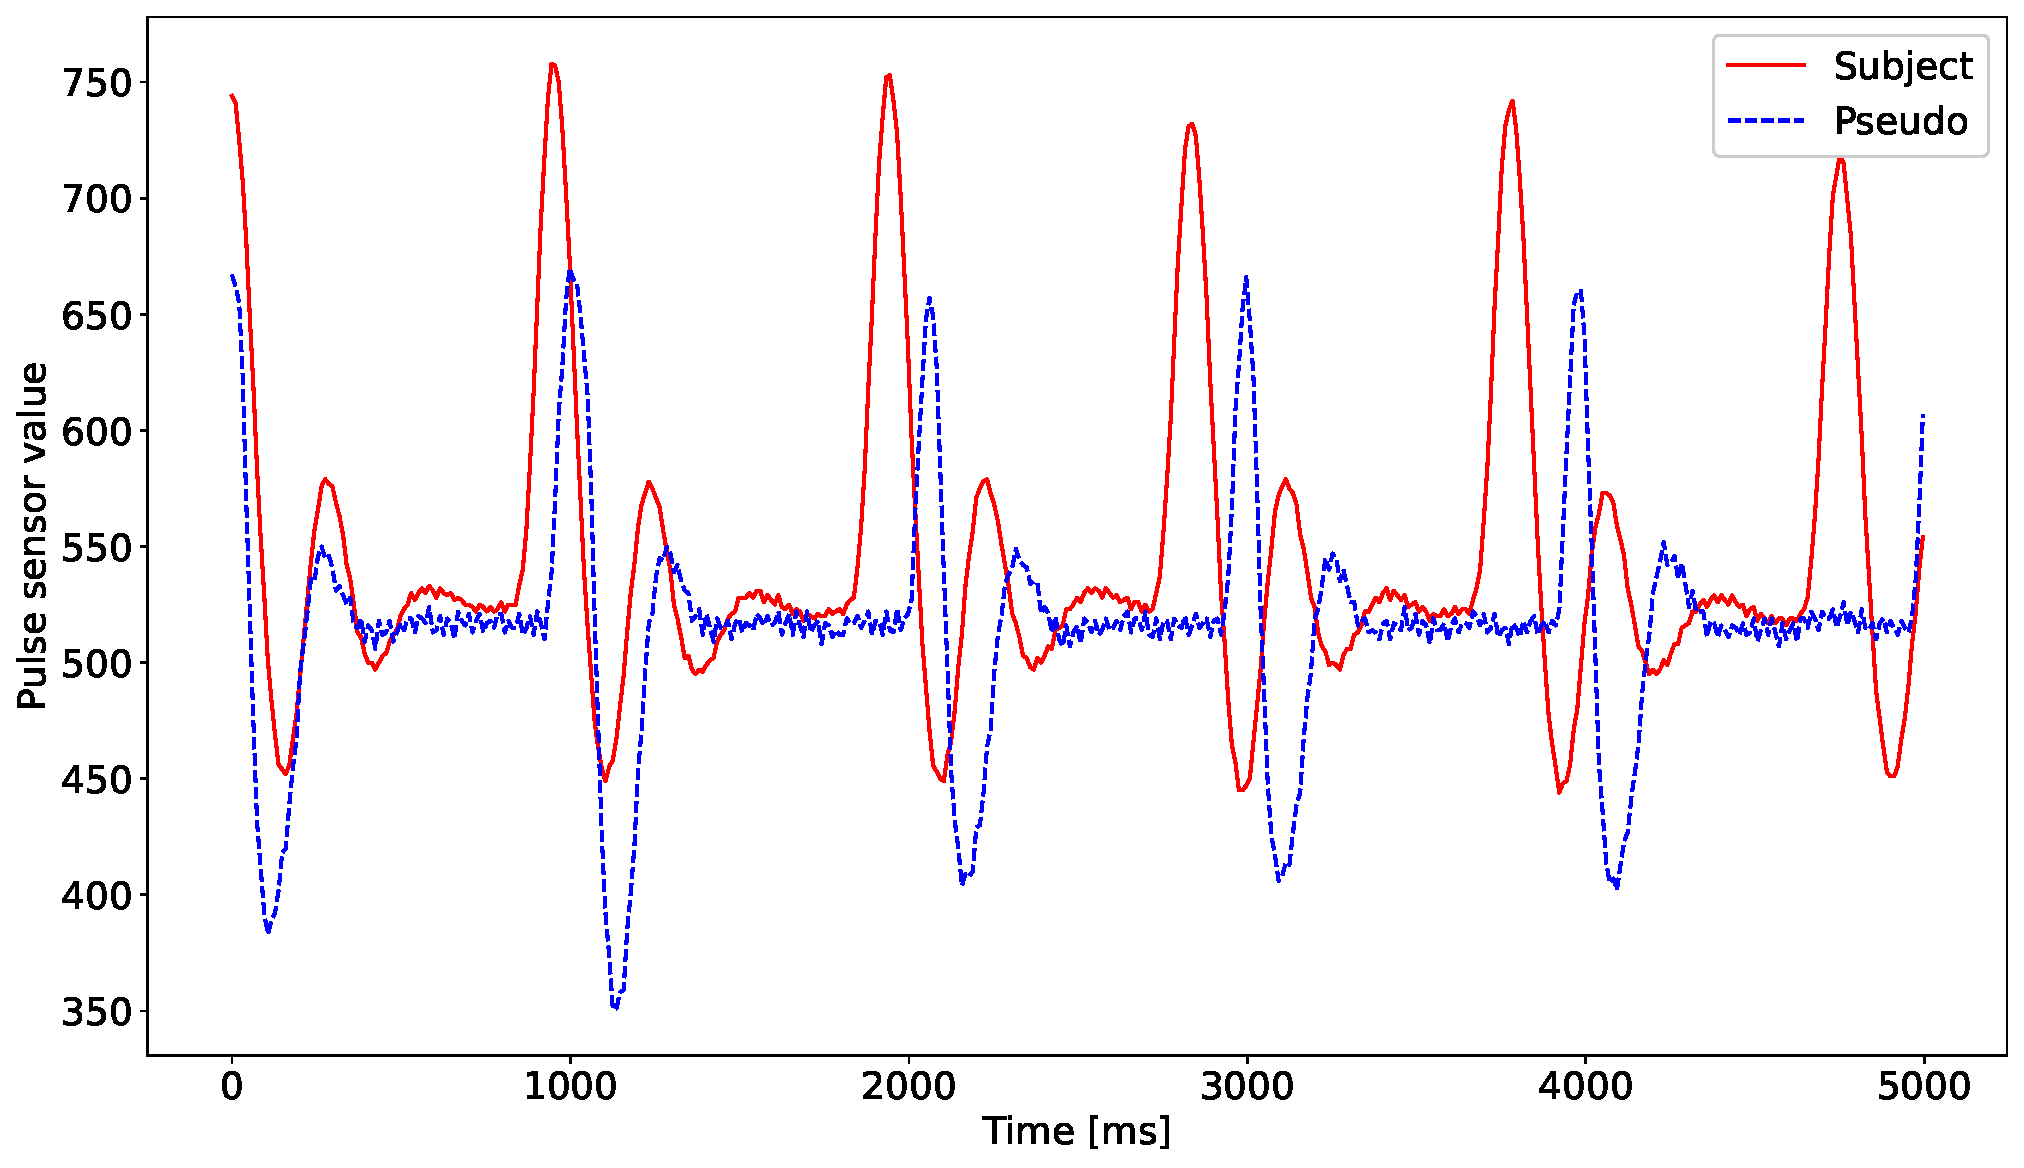
\includegraphics[width=1\linewidth]{pulse.eps}
  \end{center}
  \vspace{-8mm}
  \caption{脈波センサの取得値の変化}
  \label{fig:pulse}
\end{figure}


\begin{thebibliography}{3}

%   \bibitem{accuracy_in_low_intensity} S. Spinsante et al.: Accuracy of Heart Rate Measurements by a Smartwatch in Low Intensity Activities, MeMeA2019, pp. 1-6 (2019).
  \bibitem{fatigue_detection} 今井ら: スマートウォッチを用いた疲労度検出の試行に関する研究, 日本知能情報ファジィ学会 ファジィ システム シンポジウム 講演論文集, Vol. 34, pp. 407-408 (2018).
%   \bibitem{arrhythmia_detection} Han et al.: Premature Atrial and Ventricular Contraction Detection using Photoplethysmographic Data from a Smartwatch, Sensors, Vol. 20, No. 19, pp. 5683 (2020).
\end{thebibliography}

\end{document}